In der Bildverarbeitung kann ein gegebenes Signal häufig nur durch eine
unstetige Funktion dargestellt werden.
Sobolev-Funktionen, obwohl im Allgemeinen nicht unbedingt stetig\todo{Quelle
für Beispiel für unstetige Funktionen sind nicht immer
Sobolev?},
lassen die oftmals benötigten Sprünge über ein-kodimensionale Mengen nicht
zu. Die Menge der Funktionen von beschränkter Variation ist 
eine echte Obermenge des Sobolev-Raums der einmal schwach differenzierbaren 
Funktionen und hat sich als geeignet für diese und weitere Anwendungen erwiesen 
\cite{ABM14, AK06, Bar15} \todo{vielleicht noch Braides hier zitieren}.

\todo[inline]{Genauer sein, also schon $\Omega$ und alles definieren? 
soll man die Sachen zitieren, wenn die Formulierung davor von diesen 
Werken inspiriert ist? Sollen noch Kapitel angegeben werden?}

Eine mögliche Problemstellung in der Bildverarbeitung ist die 
Rauschunterdrück\-ung, das heißt der Versuch unerwünschtes Rauschen in einem
Signal zu verringern. Das ROF-Modell ist ein Modell-Problem dafür und sucht
eine Funtion $u:\Omega\to\Rbb$ die das Funktional
\begin{align*}
  I(u)\coloneqq |u|_{\BV(\Omega)}+\frac{\alpha}{2}\Vert
  u-g\Vert_{L^2(\Omega)}^2
\end{align*}
minimiert,
wobei $g\in L^2(\Omega)$ das gegebene verrauschte Bild beschreibt und 
$\alpha\in \Rbb_+$ ein Parameter ist, mit dem gewichtet werden kann, wie 
stark Oszillationen minimiert werden sollen, beschrieben durch den Term
$|u|_{\BV(\Omega)}$ und wie nahe die Lösung $u$ an der Eingabe $g$ liegen
soll, beschrieben durch den Term $\Vert u-g\Vert_{L^2(\Omega)}$.
Wie in \Cref{fig:exampleDenoising} zu sehen, führt die Wahl von einem zu
kleinen $\alpha$ zu einer zu glatten, verwaschen aussehenden Lösung [ref Abb c
später oder vlt noch was anderes, wenn mehr Bilder dazu kommen] während die 
Wahl von einem zu großen $\alpha$ das Rauschen kaum verringert [ref
das entsprechende Subbild].

Benannt ist das ROF-Modell nach Rudin, Osher und Fatemi, die dieses 
Problem 1972 in \cite{ROF92} vorschlugen
[cite Getreuer, Chambolle-Pock 2011, bartelsErrorControlAndAdaptivityForBV].

\bigskip
------------------------
write the introduction similar to
[bartelsErrorControlAndAdaptivityForBV], just more details. See below.

In particular, drop infos needed about BV (wir werden sehen, dass BV Funktionen
dies und das erfüllen und deshalb diese und jene Terme definiert sind)
or (wir werden zuerst grundlagen einführen aus der Optimierung und über BV 
Funktionen [dann verweis auf das entsprechende Kapitel], anschließend
das konitnuierliche Problem betrachten [verweis auf kapitel] \ldots)
\bigskip

1. BV Funtionen allgemein: lassen unstetigkeiten zu, mehr als Sobolev 
Funktionen,
[hier nochmal überlegen, wie ich dieses über 'manifold' (one codimensional
(ABM)) springen schreibe, ohne ins Detail gehen zu müssen]
\medskip

deshalb Anwendung zum Beispiel in
\medskip

[\cite{ABM14} modelization of a large number of problems in physics, mechanics,
or image processing requires the introducion of new functionals spaces
permitting discontinuities of the solution. In phase transitions, image
segmentation, plasticity theory, the study of crasks and fissures, the study of
the wake in fluid dynamics , and so forth, the solution of the problem presents
discontinuities along one-odimensionalmanifolds.
-solution of these problems cannot be found in classical Sobolev spaces
\medskip

Viele physikalischen Anwendungen können mit kontinuierlichen Funktionen nicht
beschrieben werden [Bartels, Error Control and Adaptivity for a variational
model problem defined on functions of bounded variation, und darin zitierte
Quellen].
\medskip

introduction aus [Braides] zitieren einfach mit Bemerkung, dass man dort
Beispiele finden kann (vielleicht auch nicht, da sie direkt auf SBV
eingeht und nicht auf BV)
\medskip

insbesondere in der 'Bildbearbeitung' (finde
noch das richtige Wort, Computer Vision, computergestützte Analyse von Bildern
oder so änhlich) wird das genutzt
(Quellen: \cite{AK06}, \ldots)

\cite{Get12} ist mglw ein guter Verweis für weitere Infos zum Denoisung und
wahrscheinlich in Kapitel 6 auch zur Wahl von alpha, sagt
aber auch viel über die Interpretation der Parameter
Wahrscheinlich auch sowas schreiben wie ,Die Anwendung ist kein zentraler
Punkt in dieser Arbeit, sonder \ldots, für weitere Details zum Denoising siehe
\ldots.' Dann im Experimente Kapitel eine kleine Rand-Section, in der geguckt
wird, wie verschiedene Alpha sich auf Denoising auswirken, rein optisch 'nur
ein kleiner experementeller Exkurs zur Wahr des Tuning Parameters alpha'

Vielleicht auch den Press Release zum Schwarzen Loch Bild erwähnen oder ist
das zu random?


\medskip

2. als Modell Problem dient das ROF-Modell (\cite[sec 6.2.1]{CP10}, beschreibt
auch,
was die Parameter und Terme sollen, aber vielleicht auch noch andere Quellen 
dazu (''siehe auch JZ13'')

\medskip
natürlich an dieser Stelle das Funktional einmal wie in Bartels hinschreiben

an der stelle vielleicht auch kurz schreiben, was Bartels tut und dann was wir
hier tun im Unterschied dazu

\medskip

benannt nach Rudin, Osher und Fatemi, die das Modell vorschlugen in
\cite{ROF92} (das ist auch aus CP10, also mit in das Zitat von CP10 rein)

\medskip
u ist die exakte Lösung, g das gesehene verrauschte Bild und alpha Gewichtet 
das Verhältniss zwischen Regularisierung und data fitting (tradeoff
between regularization and data fitting, CP10)
(zitiere eines der Paper/Bücher, CP10 above klärt das ganz gut)
große alpha wenig Entrauschen, kleine alpha blurry, oversmoothed u
\cite{JZ13}

\medskip
TV Term verringert Oszillationen, lässt aber Unstetigkeiten der Lösung zu.
Regularisierungs Term, der Rauschen und kleine Details entfernt.

\medskip
der zweite Term versucht die Lösung nahe an g zu halten (Treue, fidelity) (cite
getreuer und JZ13, hat aber keinen mathscinet entry), vielleicht auch nur
für mich

\medskip
INSBESONDERE erst ROF beschreiben und Parameter erklären und dann CCs 
Variante hinchreiben

\medskip
3. wir betrachten hier eine leicht abgewandlete Variante, die wie folgt
zusammenhängt (dann dieses Remark (aber wohl nicht mehr als Remark)

\begin{remark}
  In \cite[Kapitel~10.1.3]{Bar15} wird \Cref{prob:continuousProblem} für ein
  gegebenes $g\in L^2(\Omega)$ formuliert
  mit dem Funktional 
  \begin{align*}
    I(v)\coloneqq |v|_{\BV(\Omega)} + \frac{\alpha}{2}\int_\Omega (v-g)^2\dx
  \end{align*}
  für $v\in \BV(\Omega)\cap L^2(\Omega)$.

  Nun wählen wir $f = \alpha g$. Dann gilt
  $I(v) = E(v) - \Vert v\Vert_{L^1(\partial \Omega)}+ 
  \frac{\alpha}{2}\Vert g\Vert_{L^2(\Omega)}^2$ für alle 
  $v\in \BV(\Omega)\cap L^2(\Omega)$. Da der Term $\frac{\alpha}{2}\Vert
  g\Vert_{L^2(\Omega)}^2$ konstant ist, haben die Funktionale $E$ und $I$ somit
  die gleichen Minimierer in $\left\{v\in\BV(\Omega)\cap L^2(\Omega)\mid 
  \Vert v\Vert_{L^1(\partial\Omega)}=0\right\}$.
\end{remark}

4. Kurzen Überblick über Aufbau der Arbeit (,,In Kap 1 machen wir das, dann das
in Kapitel 2, dann das in Kapitel 3, \ldots``)

5. auch ein hübsches Bild wie bei Philipp (siehe Paper, sowas wie: Originalbild 
links, verrauschtes Bild (Art des Rauschens nennen) mitte, entrauschtes Bild
rechts). Falls ich die Experimente so eingestellt bekomme, dass sie entrauschen
 (todo)

\begin{figure}
  \centering
  \begin{subfigure}[b]{.4\linewidth}
    \caption{\url{https://homepages.cae.wisc.edu/~ece533/images/cameraman.tif}}
    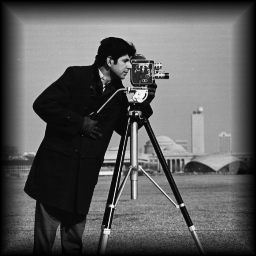
\includegraphics[width=\linewidth]{pictures/introBeta/cameraman.png}
    \label{fig:camerman}
  \end{subfigure}
  \quad
  \begin{subfigure}[b]{.4\linewidth}
    \caption{$\snr=10$}
    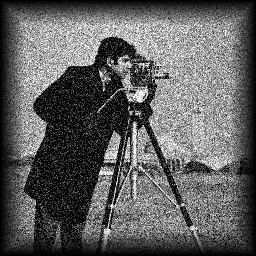
\includegraphics[width=\linewidth]{pictures/introBeta/snr10.png}
    \label{fig:camermanSNR10}
  \end{subfigure}

  \begin{subfigure}{.3\linewidth}
    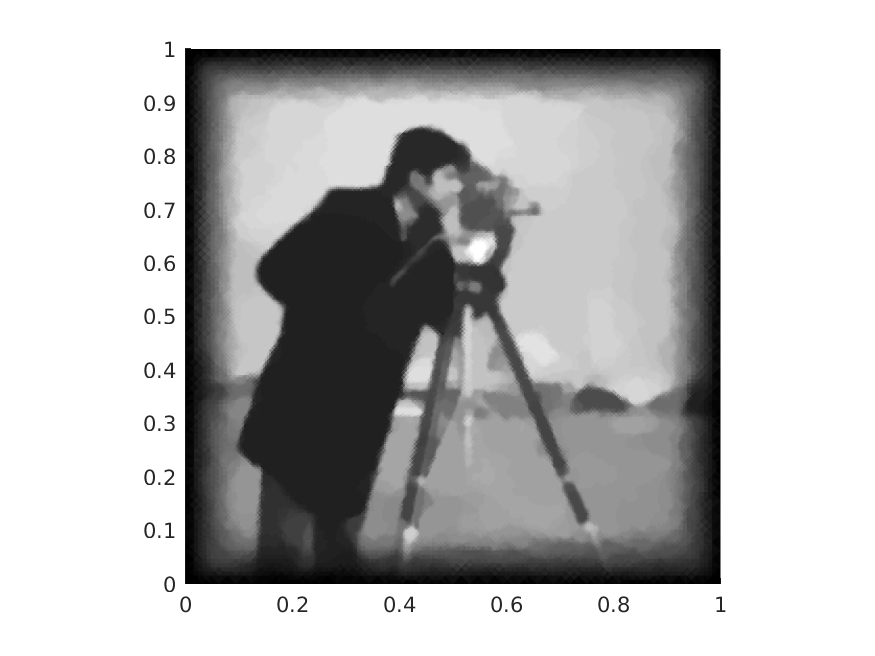
\includegraphics[trim = 60 0 60 20, clip, width=\linewidth]
      {pictures/introBeta/snr10/01000.png}
    \caption{$\alpha=1000$}
    \label{fig:snr10alpha1000}
  \end{subfigure}
  \begin{subfigure}{.3\linewidth}
    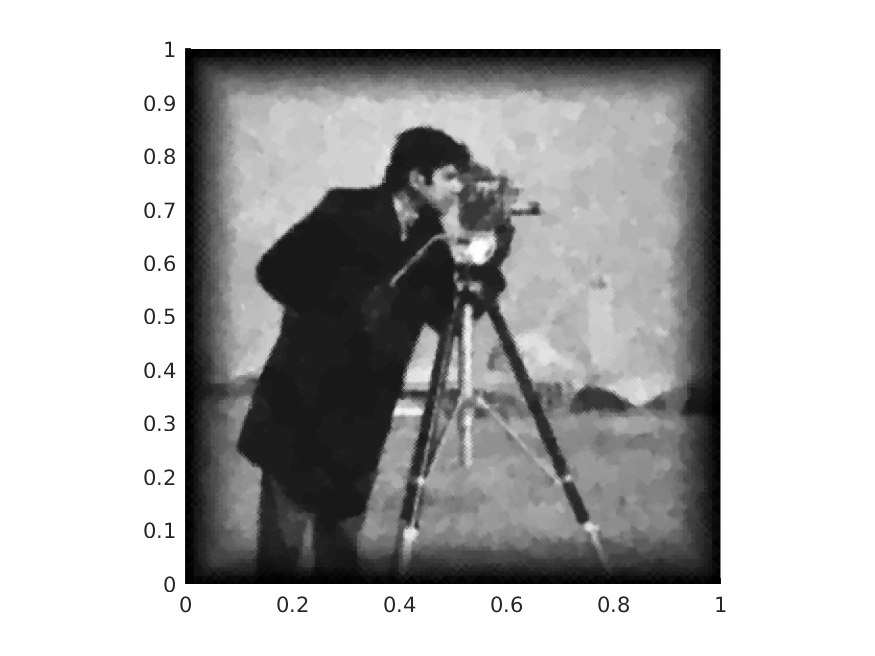
\includegraphics[trim = 60 0 60 20, clip, width=\linewidth]
      {pictures/introBeta/snr10/02500.png}
    \caption{$\alpha=2500$}
    \label{fig:snr10alpha2500}
  \end{subfigure}
  \begin{subfigure}{.3\linewidth}
    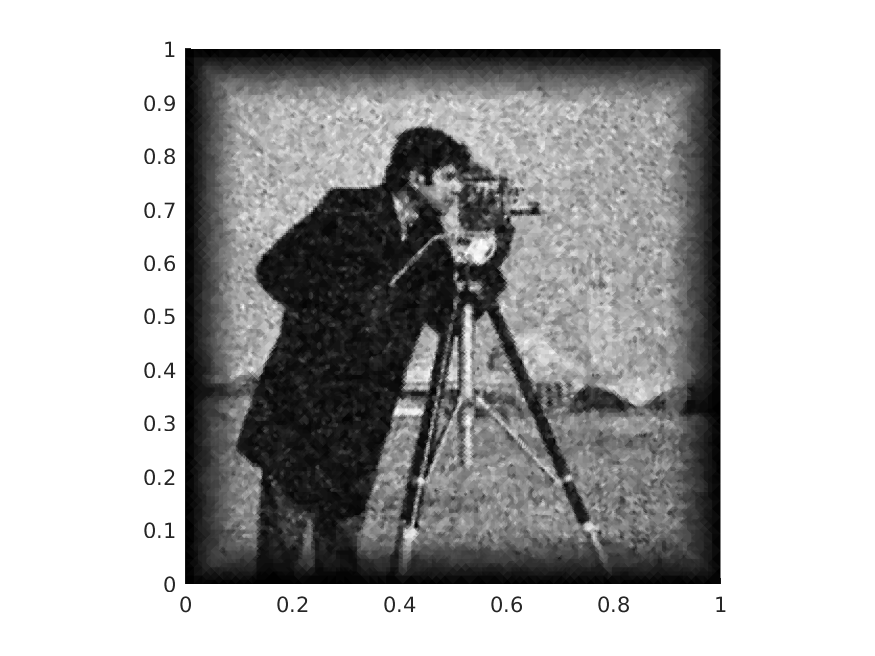
\includegraphics[trim = 60 0 60 20, clip, width=\linewidth]
      {pictures/introBeta/snr10/10000.png}
    \caption{$\alpha=10000$}
    \label{fig:snr10alpha10000}
  \end{subfigure}
  \caption{Originalbild (a) und Originalbild mit additiven weißen gaußschen
  Rauschen (b) mit einem Signal-Rausch-Verhältnis (eng.\ signal-to-noise
  ratio, SNR) von 10, jeweils mit nachträglich hinzugefügten graduellen
  Übergang zu schwarzen Rand, was Nullranddaten entspricht und drei Ergebnisse
  (c)-(d) des adaptiven Algorithmus mit verschiedenen Werten von $\alpha$}
  \label{fig:exampleDenoising}
\end{figure}

\begin{figure}
  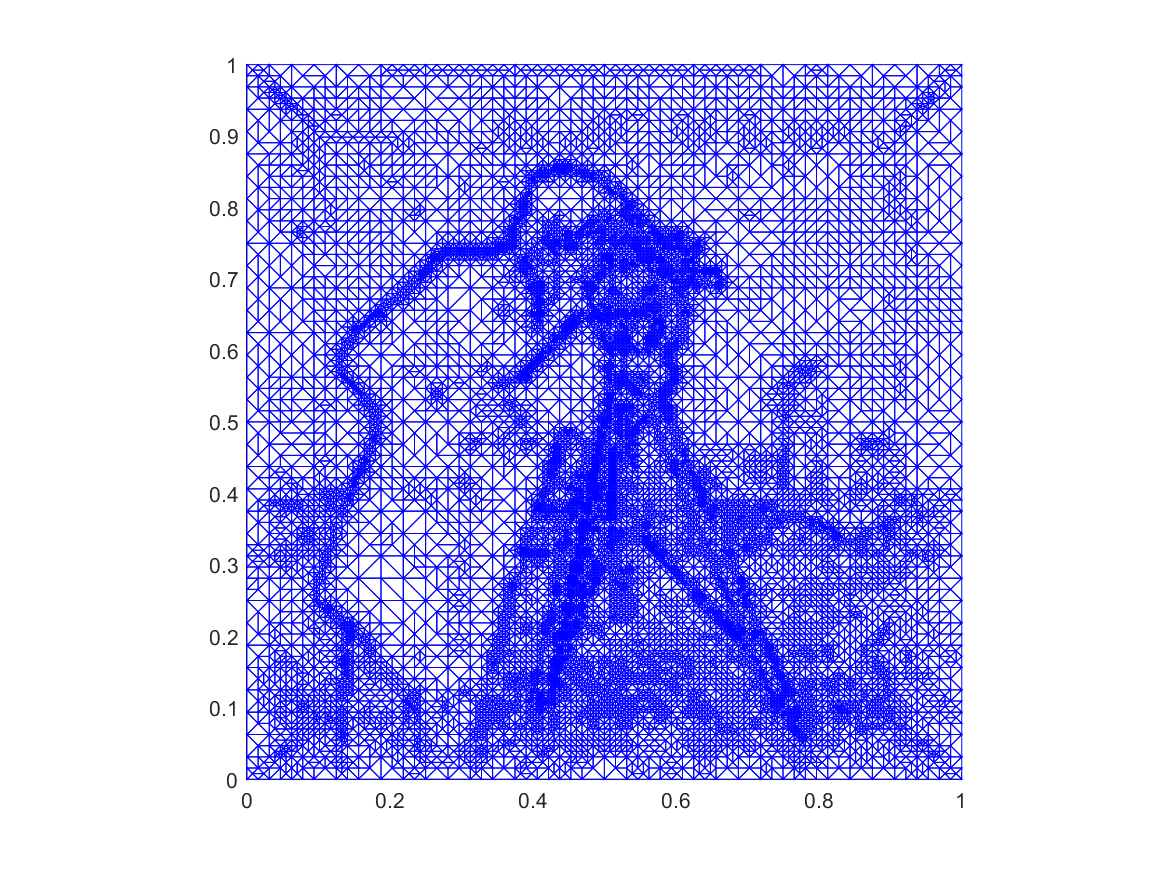
\includegraphics[trim = 60 0 60 0, clip, width=\linewidth]
    {pictures/introBeta/triangulation/triangulation.png}
  \label{fig:exampleTriangulation}
  \caption{Triangulierung mit 40300 Freiheitsgraden erzeugt vom adaptiven
  Algorithmus für rauschfreien Input}
\end{figure}

